\documentclass[a4paper]{article}
%article
%report

\usepackage{listings} % for importing code

%math formatting with $...$
\usepackage{amsmath}
%math font, $\mathbb{...}$ will be big, double-lined letters for sets
\usepackage{amssymb}

\usepackage{subfiles}

\usepackage{float}

\usepackage{graphicx}
\usepackage{framed}

\usepackage{pgfplots} % requires texlive-pictures to compile


\usepackage{xparse} % allows optional arguments on self defined commands

\usepackage{multicol}

\usepackage[bookmarks]{hyperref}
\setlength\parindent{0pt} % sets indent to zero

\newcommand{\horiz}{\begin{center}\line(1,0){400}\end{center} } % draws a horizontal line.
\newcommand{\smallhoriz}{\begin{center}\line(1,0){400}\end{center} } % draws a horizontal line.





%format margins
%1.5in is about default, .5in is giant, 1.0 is slightly too wide, 1.2 looks like word
\usepackage[margin=1.2in]{geometry}

\begin{document}

\title{CMPE-240 \\ Final Project}
\date{\today}
\author{Henry Zimmerman}
\maketitle



\section{Abstract}\label{sec:abstract}
The project as proposed set the objective of being able to unlock a door remotely using a Raspberry Pi, a servo, and an Android Wear SmartWatch.
To complete this objective, pulse width modulation, backend web development skills, and abuse of Google's speech-to-text system were utilized.
While the finished project was not mounted to a door's lock, the project did demonstrate capabilities indicative of meeting its objective of remotely unlocking a door.

\section{Design Methodology}\label{sec:designMethodology}

A proposal was initially drafted which specified that the software for the project would require a webserver, a controller for the servo, an Android Wear App and an Android phone service.
The proposal also listed the required hardware to meet the objective.
This included:
\begin{enumerate}
    \item Raspberry Pi
    \item Power source (Pi)
    \item Router
    \item Android Wear SmartWatch
    \item Servo
    \item Battery (Servo)
    \item 40 Pin Breakout Cable
    \item Breadboard
    \item Wires
\end{enumerate}

Implementation of the project began with the webserver.
Because it was known that controlling the servo was a time sensitive affair, Rust was chosen as the language for the server.
Rust is new language developed within the last decade with the goal of supplanting C with something just as fast, but prone to fewer runtime errors.
The design called for the webserver to talk to the servo controller, so the choice was made to keep both of those components in the same language and as part of the same program.
Rust's lack of garbage collection, instead opting for a compile-time lifetime tracking system, inspired confidence that servo control would not be interrupted by GC pauses.
Initially, Rust's promise of being able to run on bare metal was appealing, as being able to write the project without an underlying OS would be consistent with other labs in CMPE 240.
The goal of running without an operating system did not come to fruition for reasons that are explained later.

Rocket, a webserver framework, was chosen to be used to write the server component, primarily because of existing familiarity with the framework.
It uses Rust's advanced macro and type systems to take very plainly written functions that represent API endpoints, and automatically convert them into other functions that will perform input validation, match expected request routes, and set up error handlers, manage server state, and other actions that usually require excessive boilerplate code.
Because of how terse the webserver code was, it took very little time to get a simple webserver that would respond with HTTP 200 for a given request, indicating a successful handling of the request.
In fact, it took longer to set up port forwarding and a domain then it did to get the initial server running.
The server was tested by using Firefox's ``Edit and Resend'' feature in the developer tools to send POST requests to the domain under which the Pi was situated.
HTTP 200 responses were observed in Firefox and \texttt{stdout} logs were observed over SSH on the Pi.


Unfortunately, in order for Rust to be able to run without an OS, every dependency in a binary or library needs to be marked with the \texttt{no\_std} attribute, and Rocket, being a large library with dependencies of its own, did not have this marker.
It was unlikely from the start that running on bare metal would be practical (getting networking working without an OS likely would have proved too difficult anyway), but this dependency issue made it clear that Raspbian was required for this project.


With an initial webserver running, it was time to attach the servo to the Pi so the controller could be tested while being developed.
The breakout cable was used to connect all 40 pins on the Raspberry Pi to the breadboard.
Because the servo requires 5V to operate, and a pin on the Pi can only provide about 3.5V, an external battery pack was required to provide power.
The servo had three wires to connect: power, ground and signal.
The battery pack was connected to the vertical power rails of the breadboard.
The servo's power and ground were attached to the respective rails on the breadboard.
The provided guide for the servo suggested connecting the signal wire to pin 18 of the Raspberry Pi, as it suggested that only this pin could be controlled with enough precision to send meaningful signals to the servo.
The guide was old and had been written for use with the Raspberry Pi 1 - Model B variant, which had fewer pins overall and it was unclear if later generations had pins that could send precise signals on all pins.
Pin 16 of the Raspberry Pi 3 was chosen with the intention of trying other pins if pin 16 couldn't be driven with enough precision to control the servo.

Figure ~\ref{fig:breadboard} demonstrates the setup of the breadboard.
It can be seen that the Pin 16 from the Pi is attached to the yellow signal cable.
Because the servo's control signal only requires 3.3 volts, the pin from the Pi is enough to signal the servo without additional assistance.
The cables from the external batteries that provide the 5v can be found at the bottom of the figure.

\begin{figure}[H]
    \center
    \caption{Breadboard}
    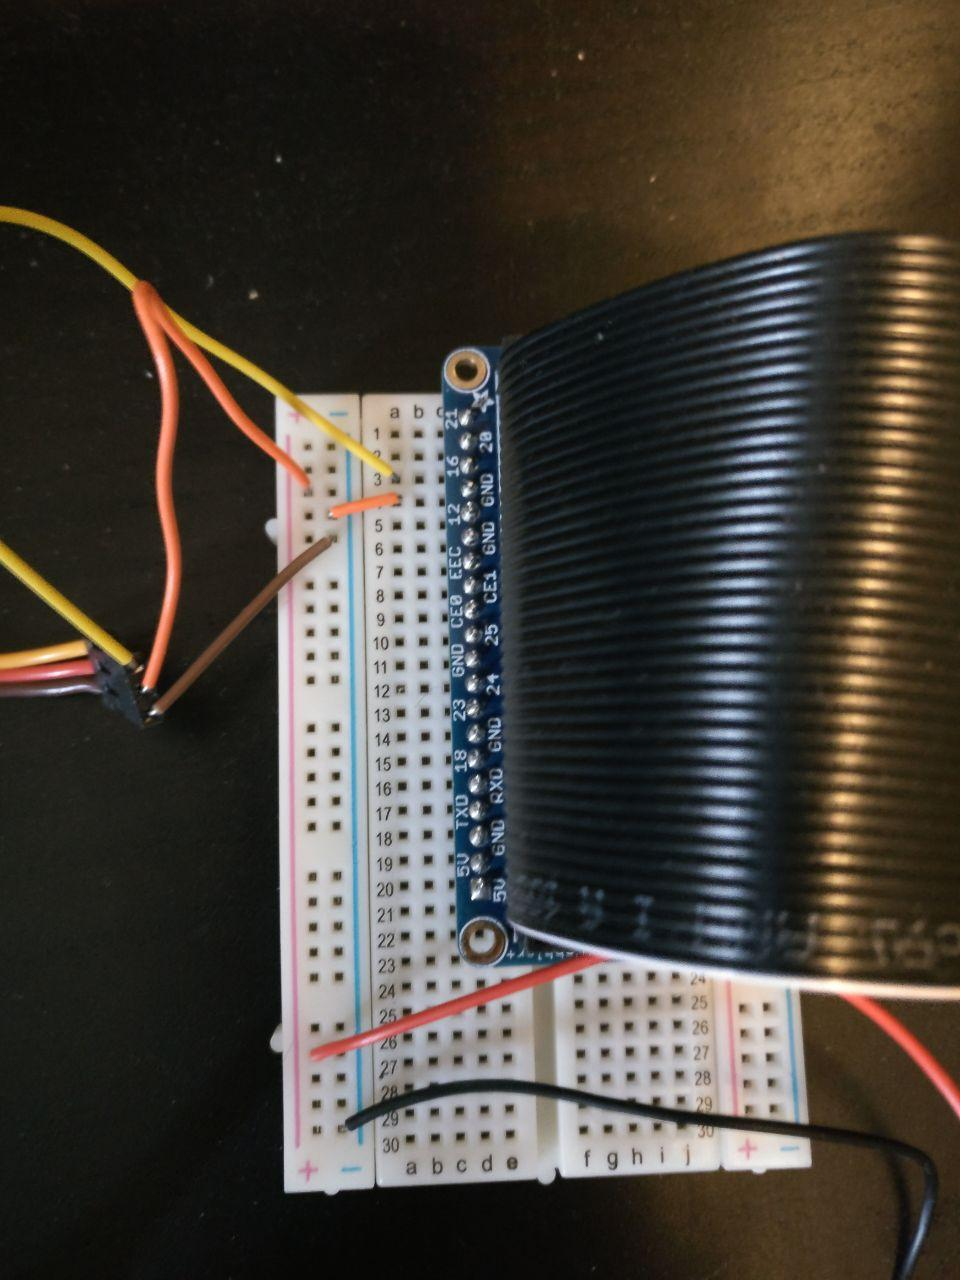
\includegraphics[width=10cm]{breadboard.jpg}
    \label{fig:breadboard}
\end{figure}



With the servo wired to the Pi, software to control the servo was required next.
The original proposal indicated that a library (called a `crate' in Rust terminology) called \texttt{cupi} could be used to control the GPIO pins of the Pi.
Unfortunately, it was found that the crate had not been maintained in 2 years and did not compile, likely due to changes to Raspbian in that time.
Instead, another crate, \texttt{sysfs\_gpio} was used to control the GPIO pins.

\texttt{sysfs\_gpio} works by passing a closure to a \texttt{Pin} instance that will spawn a separate thread to control the GPIO pin.
The closure in question would contain code that would control the pin's state for the time the thread was alive.
This setup has the advantage of allowing code inside the closure to \texttt{panic!()}, a safer alternative to segfaulting, that would cause the thread in question to die without bringing down the rest of the server program.

The graceful failing with \texttt{panic!()} was useful in tracking down a bug.
When the closure executes, it would need to configure the pin before setting it high or low.
If it couldn't, it would \texttt{panic!()} by calling \texttt{expect()}, causing the thread to crash.
Apparently, the \texttt{Pin}'s function that takes the closure first tries to set the pin to allow configuration before executing the closure, but the \texttt{udev} system, which is responsible for device permissions on Linux, would take too long to set.
This caused the closure to try to configure the pin before the OS had granted access to do so, causing the error.
Because \texttt{expect()} could be called on a function that may return an error, an error message was able to be included that would indicate which function was responsible for this error.
This problem was resolved by adding a 100 ms delay before the pin was configured, allowing udev to do its thing before the pin was manipulated.


Once accessing GPIO pins ceased causing the servo thread to crash, determining if controlling the servo was possible was the next task.
Based on Figure \ref{fig:servo}, it was apparent that the servo would expect a signal pulse every 20 ms, and the servo would rotate to an angle that corresponds to the pulse width.



This technique for controlling hardware in this manner is known as pulse width modulation, or PWM.
The initial implementation of the function that would send the pulses would set the pin low, wait for 20 ms, set it high, and then wait for 1 or 2 ms, and this would repeat for about a second.
Surprisingly, this worked on the first try, but the servo experienced some jitter where it would reach its expected angle, but would move 10 degrees in either direction once there until the looping stopped.
This was solved by setting the pin low, waiting for 20 ms \emph{minus} the pulse duration, then setting it high, and waiting out the pulse duration.
This led the period to always be 20 ms, instead of 21 or 22 ms as it was initially implemented.
Because the pulse period was closer to what the servo expected, the jitter disappeared and the servo worked as expected, rotating about 90 degrees, enough to move a door lock between the unlocked and locked positions.
The time it took for the servo to rotate into place was eventually ascertained to be less than a second, so the 20 ms pulse was repeated 40 times, causing the PWM loop to take about 800 ms to execute.


The pulse sending function was included with a Struct representing the servo that held the \texttt{Pin} instance and an Enum that indicated which orientation the servo was in.
A toggle function was provided that would move the servo between the locked and unlocked positions every time it was called.
The servo struct was then initialized in the main body of the server, wrapped in a Mutex to enforce synchronous access, and then managed by the Rocket server, so that it could be given to the endpoint function so it could be toggled when a request was received that matched the endpoint.


Once the server and servo were working as expected, the only remaining component was the watch client.
The proposal assumed that a companion service was required to run on the phone to provide networking to the WAN, as that scheme was required for Android Wear 1.X.
It was discovered in the process of creating the app that Android Wear 2.0 supports sending network messages directly from the watch, which would then either use the watch's own WiFi connection, or proxy through the phone via its persistent bluetooth connection automatically.
It was simple to set up an activity (Android term for a UI thread) that would send a request to the Pi when the app started.
When the watch received a HTTP 200 response from the Pi, it would change its displayed text to let the user know that the lock had toggled position.
If the Pi encountered an error, or the request couldn't make it to the Pi, the Wear app would change its text to indicate that an error had occurred.
At this time, the servo was controllable via the watch, but it lacked the voice command specified in the proposal.

Setting up a voice command was obtuse.
The app was originally called ``Sesame'' because Android Wear supports opening installed applications by saying ``Ok Google\ldots Open APPNAME''.
The chance at clever wordplay was the inspiration behind this project.
Despite significant effort, it was impossible convince Google's speech-to-text (STT) engine and internal app name lookup system to open an app named ``Sesame'' with voice commands.
The name of the app used for lookup via Google's STT system was changed to ``Lock'', after which, the command ``Open Lock'' would reliably open the Sesame app, causing the POST request to be sent to the Pi.


\section{Results and Analysis}\label{sec:resultsAndAnalysis}
With the required components completed: the server, servo wiring, servo controller logic, and Android Wear app, it was now possible to rotate a servo by remotely speaking a voice command.
The server would toggle the servo, and log this information.
A sample server log of Rocket starting and handling requests for toggling the servo is provided in Figure \ref{fig:logs}.
This demonstrates that the server is capable of handling requests and altering its representation of the servo across multiple requests.

\begin{figure}[H]
    \center
    \caption{Server Logs}
    \label{fig:logs}
    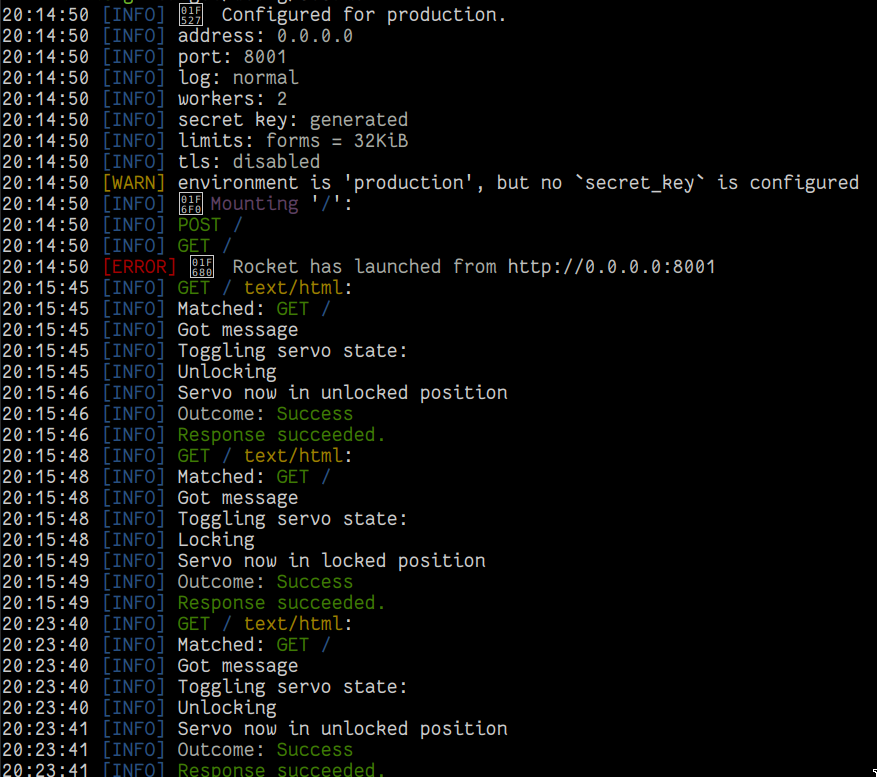
\includegraphics[width=10cm]{sesameServerOutput.png}
\end{figure}

The initial observed shaking of the servo indicated something was wrong.
There were concerns about trying to control the servo from a process running in an OS.
It might not have worked because context switching performed by the OS might have caused the thread controlling the servo to pulse or rest for too long.
This would have led the servo to jitter, as the pulses would instruct the servo to rotate to a slightly different angle every time the thread suspended for too long.
There were also concerns about Rust taking too long to execute causing inconsistencies in the servo signal, but this was disproved when no observable difference was detected when controlling the servo with an unoptimized build and a release build.
The release build for Rust is typically much faster than the unoptimized build, so if the language was at fault, a difference in servo behavior would have been noticeable between builds.
This might have been a problem in other languages with more variable runtime performance, but the lack of garbage collection means that Rust typically has consistent performance
Ultimately, it was found that the delay used to keep the pin low was leading to the full period of the pulse being too long (20 ms + pulse width), causing the servo receive a signal it couldn't adequately translate to a rotation angle.

Figure \ref{fig:servo} demonstrates how the servo is controlled.
By changing how long the pulse is, in the case of this project, between 1 ms to 2 ms, the Raspberry Pi was able to instruct the servo to change its rotation.
\begin{figure}[H]
    \center
    \caption{Servo Operation}
    \label{fig:servo}
    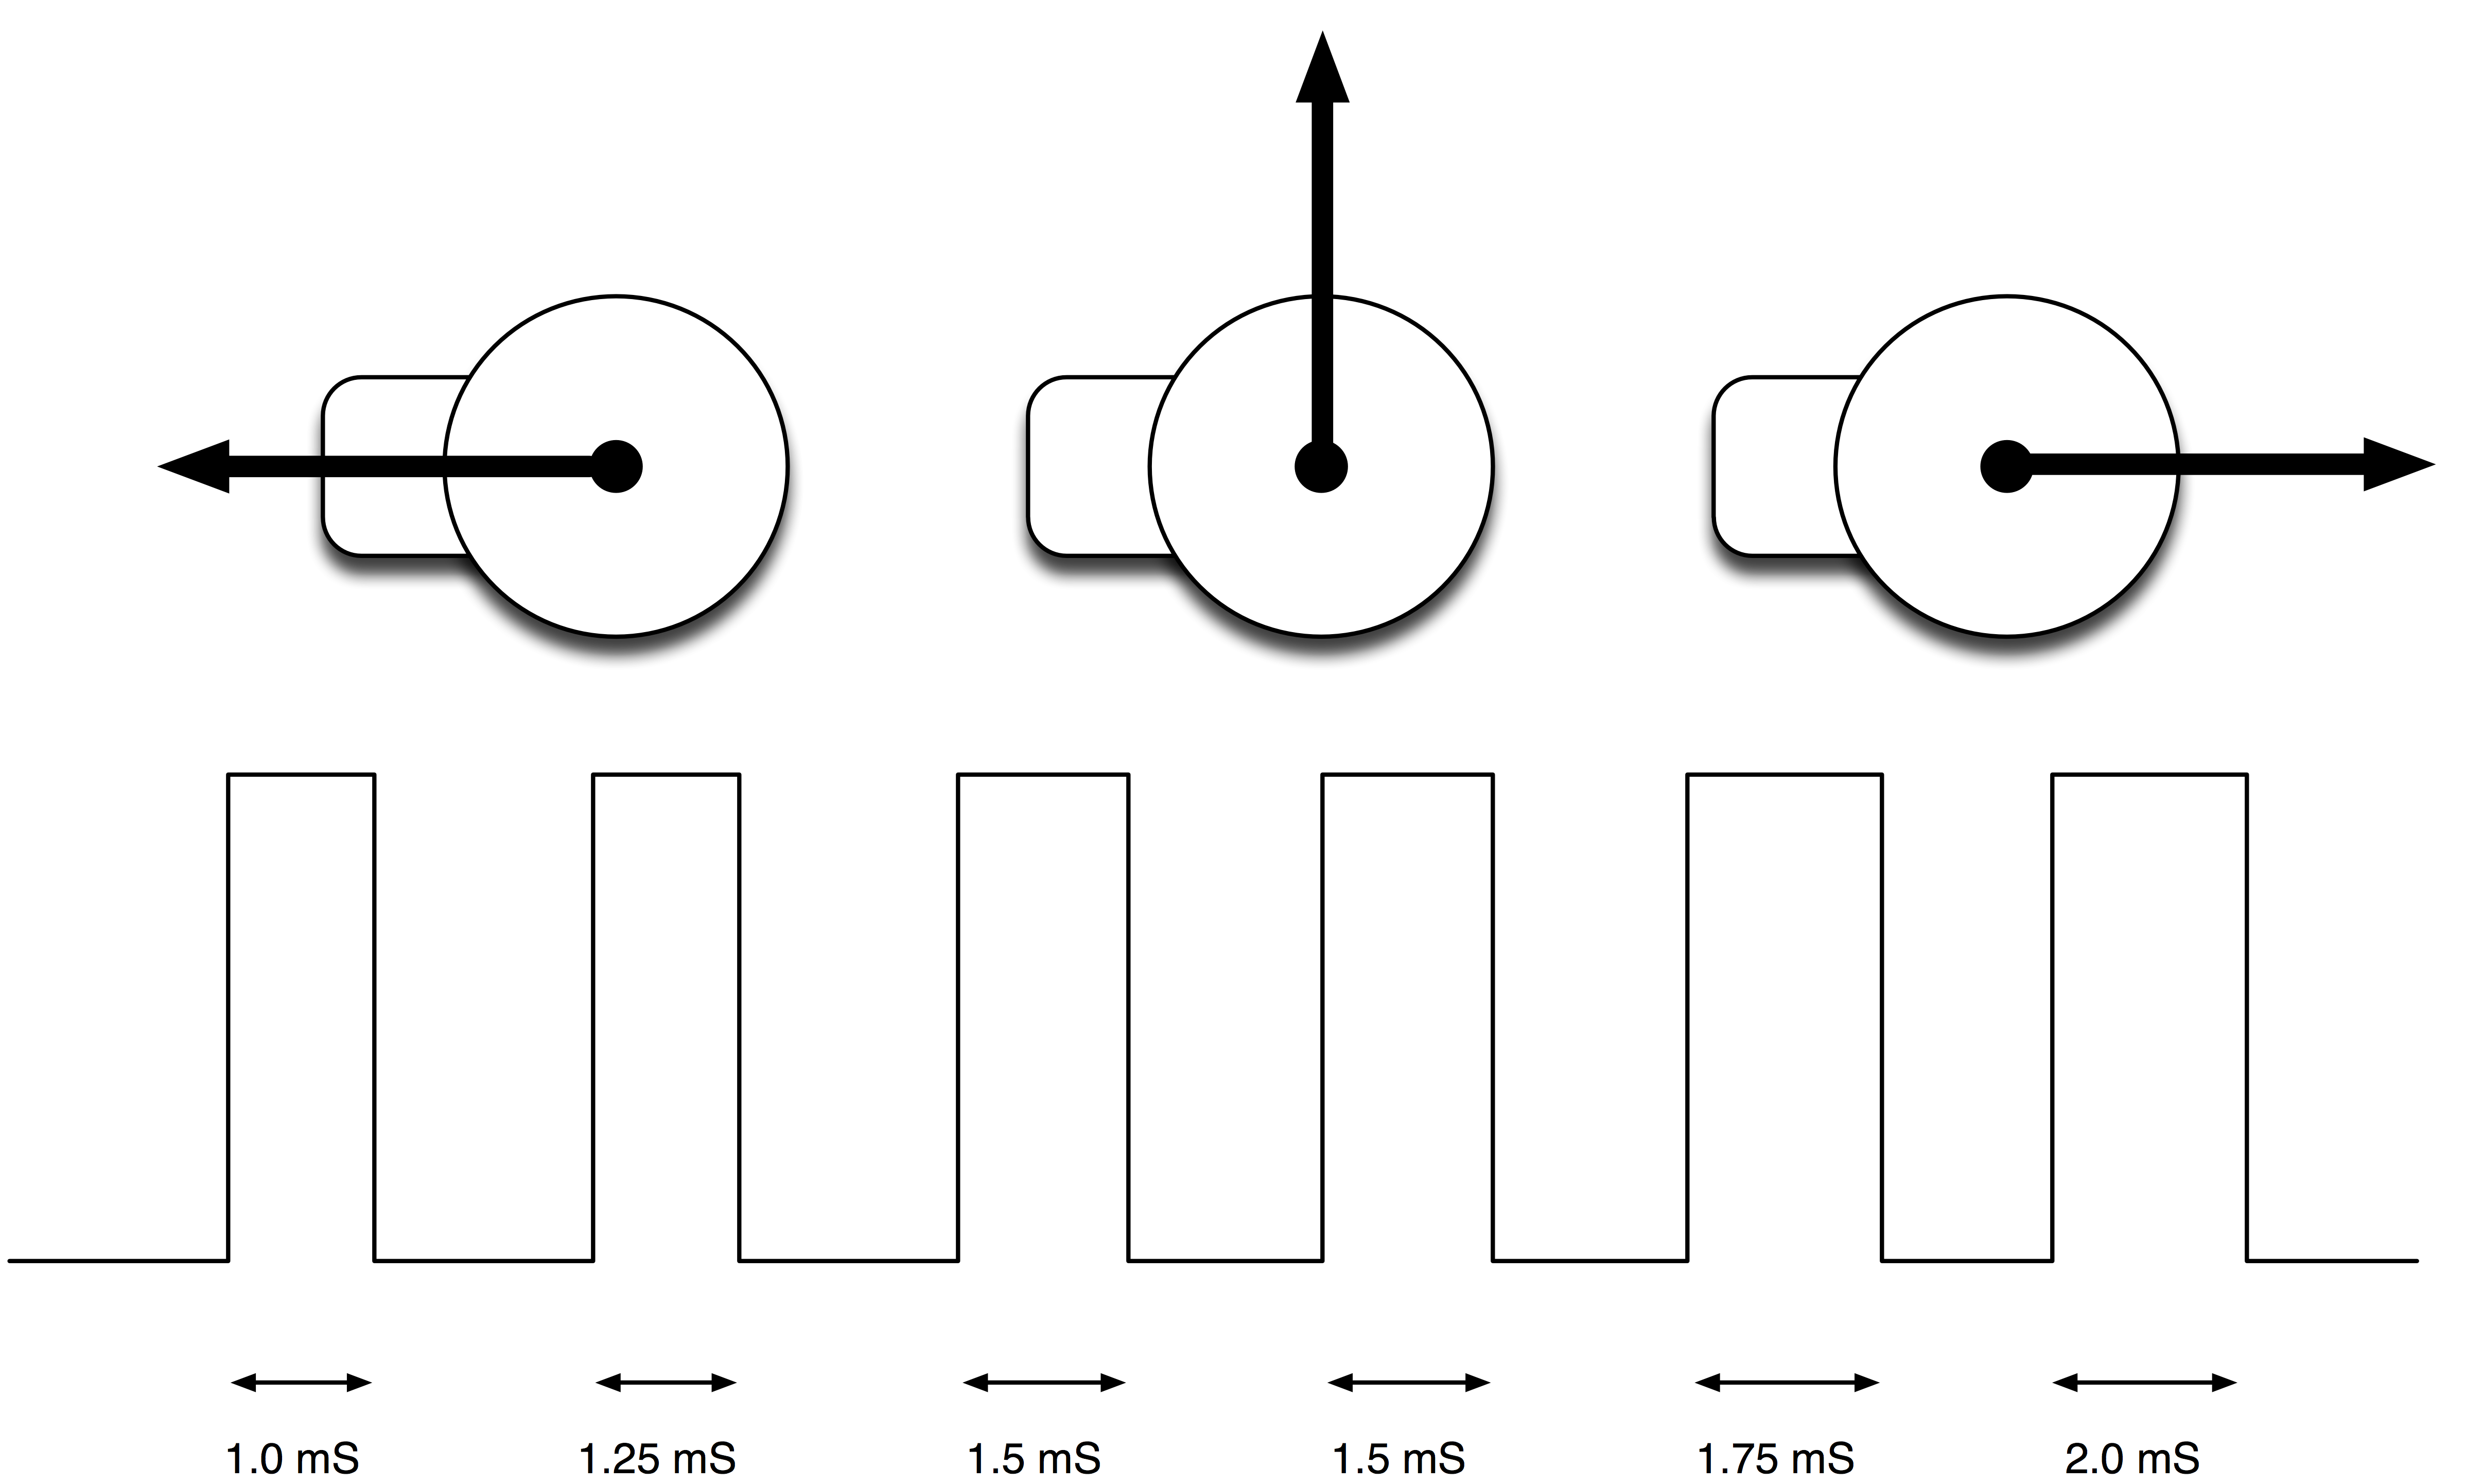
\includegraphics[width=12cm]{servoOperation.png}
\end{figure}

While Android Wear 2.0 has the ability to send network requests, it couldn't send requests to the local network, likely because it routes the requests through Google before sending them to the intended destination.
This required setting up a domain for the domicile in which the Pi was located and port forwarding requests received on port 8001 to the Pi at the local address 192.168.1.74.
Once this was done, the SmartWatch was able to send messages to the Pi.

Because the server had to be publicly accessible, and that couldn't reasonably be done on RIT's network, it was not feasible to demonstrate this project in a class presentation.
Instead, a video showing the Android Wear app being opened with voice commands, and the servo subsequently moving in response served as evidence that the project's acceptance criteria was met.
This video will be included as a separate file submitted with this project.

A sequence diagram was constructed to demonstrate how the components talked to each other, shown in Figure ~\ref{fig:sequence}.
Google's speech-to-text engine would listen for ``Open Lock'', causing the app to open, sending a request to the Rocket server running on the Pi which would then toggle the servo, causing an HTTP 200 response to be sent back to the app.
\begin{figure}[H]
    \center
    \caption{Sequence Diagram}
    \label{fig:sequence}
    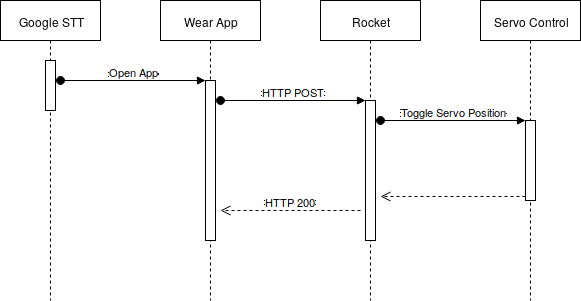
\includegraphics[width=14cm]{SesameSequenceDiagram.png}
\end{figure}



\section{Conclusion}\label{sec:conclusion}

Some opportunities that would have expanded the scope of the project were missed.
Beyond just setting up an API endpoint for toggling the lock, it would have been nice to set up other endpoints that could have switched the servo into an unlocked position, and after a specified time, lock it again.
Endpoints could have been set up to allow verified friends or acquaintances to text a Twilio number that would cause the lock to unlock for them.
A subroutine could be set up to periodically make sure that the servo is in the position the server thinks it is, and rotate the servo if it isn't.
This would allow end users to unlock it manually with a key, and know that it will lock again soon after.


While the primary goal of speaking a command to a watch to cause a servo to rotate in a manner that could unlock a door was met, a number of optional details laid out in the proposal were not met.

Due to time and material constraints, as well as a desire to get my security deposit back, it was decided that the servo would not be mounted to a door.
This would likely have required some glue to attach the servo's head to the lock, something to affix the servo's body statically to the door, as well as something to hold the Raspberry Pi and the other related circuitry.
It was too much effort for a requirement that was made optional in the proposal.

The Android Wear app was originally planned to be written in Kotlin, a JVM language that works on Android platforms.
The decision to use Java instead was motivated by the simplicity of modifying some provided example code in Java instead of learning a whole new language just to send a message over the network using minimal available documentation.

The server was originally intended to run on bare metal, but it quickly became obvious that it would not work due to dependency issues within Rust's packaging ecosystem.
The decision to use an OS instead thankfully did not impact the performance of the servo as it related to this project.


Despite the alterations that had to be made to accommodate the discrepancies between the proposal and the modern state of the software (and the door) in question,
it was found that implementing a voice controlled door lock is possible using the aforementioned materials.


\section{Source}\label{sec:source}
The relevant parts of source are made available here.
Additionally, the project itself will be hosted on Github \href{https://github.com/hgzimmerman/CMPE-240-Sesame-Server}{here} for at least the duration of the grading period and will not be modified after the due date.

\subsection{Rocket Server and Servo Control}\label{subsec:server}

\lstinputlisting[
    frame=single,
    basicstyle=\small,
    breaklines=true,
    numbers=left,
    caption=src/main.rs,
]
{../src/main.rs}

\lstinputlisting[
    frame=single,
    basicstyle=\small,
    breaklines=true,
    numbers=left,
    caption=src/servo.rs,
]
{../src/servo.rs}


\lstinputlisting[
    frame=single,
    basicstyle=\small,
    breaklines=true,
    numbers=left,
    caption=Cargo.toml,
]
{../Cargo.toml}

\lstinputlisting[
    frame=single,
    basicstyle=\small,
    breaklines=true,
    numbers=left,
    caption=Rocket.toml,
]
{../Rocket.toml}

\subsection{Android Wear}\label{subsec:androidWear}
\lstinputlisting[
    frame=single,
    basicstyle=\small,
    breaklines=true,
    numbers=left,
    caption=android/Sesame2/app/src/main/java/com/example/hzimmerman/sesame/ToggleServoActivity.java,
]
{../android/Sesame2/app/src/main/java/com/example/hzimmerman/sesame/ToggleServoActivity.java}

\lstinputlisting[
    frame=single,
    basicstyle=\small,
    breaklines=true,
    numbers=left,
    caption=android/Sesame2/app/src/main/AndroidManifest.xml
]
{../android/Sesame2/app/src/main/AndroidManifest.xml}


\end{document}
